\documentclass[a4paper]{article}

\usepackage[english]{babel}
\usepackage[T1]{fontenc}
\usepackage[utf8]{inputenc}
\usepackage{amsmath}
\usepackage{graphicx}
\usepackage{lmodern}
\usepackage[left=3cm, right=3cm, bottom=4cm, top=4cm]{geometry}
\usepackage{array}
\usepackage{listings}
\usepackage{sidecap}
\usepackage{hyperref}
\usepackage{tipa}
\usepackage{multirow}
\usepackage[gen]{eurosym}
\usepackage{float}
\usepackage{color}
\usepackage{pifont}
\usepackage{pdfpages}
\usepackage{enumitem}
\DeclareUnicodeCharacter{20AC}{\euro{}}

\usepackage{hyperref}
\hypersetup{
    colorlinks,
    citecolor=black,
    filecolor=black,
    linkcolor=black,
    urlcolor=black
}

\newcommand{\emptypage}[0]{\newpage\thispagestyle{empty}\null\newpage}

\begin{document}
    \hypersetup{pageanchor=false}
    
\includepdf[page=1]{figure/cover.pdf}
    \hypersetup{pageanchor=true}

    \newpage
    \thispagestyle{empty}
    \mbox{}

    \newpage

    \setcounter{tocdepth}{2}
    \tableofcontents
    \setlength{\parskip}{10pt}

    \newpage
    \thispagestyle{empty}
    \mbox{}

	\newpage
    \section{Special thanks}
\label{sec:thanks}

First of all, I would like to thank Michel {\sc Visser} and Simone {\sc Potenza}, co-founders of Konnektid, for hiring me as a trainee in their company.
I address special thanks to Simone {\sc Potenza}, for his precious advising and help as my supervisor.

I am also very grateful for the good work atmosphere, the mutual aid, and all the nice moments spent together with the Konnektid team.

Furthermore, I would like to thank Bruno {\sc Arnaldi}, my referent teacher during this traineeship, for his availability and helpful feedback.

Finally, I thank my engineering school: the \guillemotleft{} Institut National des Sciences Appliquées \guillemotright{} (INSA) of Rennes,
and more specifically the Computer Science department, for the knowledge acquired during my formation but also for allowing me to conduct such an interesting internship.


    \newpage
    \section{Company presentation}
\label{sec:company}

Konnektid is a startup, founded in January 2013 by Michel {\sc Visser}, the current Chief Executive Officer (CEO),
with the goal of transforming neighborhoods into universities. A few months later, Simone {\sc Potenza} joined the project
as co-founder and Chief Technology Officer (CTO). The company's website, \url{https://www.konnektid.com/}, was live in April 2014.

\subsection{Concept}
\label{ssec:concept}

Konnektid is a skill-sharing platform, empowering life-long learning and community building. It connects people who want to learn with people who can teach, and who live nearby.
This last condition is what makes Konnektid special: people find each other online, but then meet face-to-face to exchange knowledge.
These offline meetings are called \guillemotleft{} konnektions \guillemotright{}.

The website features a slogan, which is \guillemotleft{} Everyone has a skill worth sharing \guillemotright{},
and a logo visible on {\sc figure}~\ref{fig:logoKonnektid}.
\vspace{1cm}

\begin{figure}[h]
    \centering
    
\includegraphics[scale=0.6]{figure/logo_konnektid.png}
    \caption{Konnektid logo, representing conversation bubbles.}
    \label{fig:logoKonnektid}
\end{figure}

Two different kinds of members can be found in the community:

\begin{itemize}[noitemsep]
    \item Professional teachers, who pay a monthly amount for using the platform;
    \item Regular members, who use the website for free.
\end{itemize}

Professional teachers pay a monthly fee to use the platform, and get an public profile featuring their name and location but also their experience and certifications.
They can create courses or workshops, which they charge for and are able to share on main social media.
Plus, they have access to the community in order to find potential students.

On the other hand, regular members use the service free of charge. They own a private profile containing their name, their location and eventually some skills that they can teach.
They can send general requests, notifying their neighbours that they want to learn something specific.
If they see that somebody offers that skill, they can also send a personal request to that person.
And if they are willing to pay, they can book courses or workshops offered by professional teachers.

\subsection{Current situation}
\label{ssec:situation}

The Konnektid team has expanded, and it has changed a lot over the years with occasional freelancers and trainees.
At the moment it consists of a dozen of people, from very different origins and backgrounds, some of them working part-time or remote.

The website has also grown, and it now counts more than 15.000 members.
These users mostly live in the Netherlands, in the big cities such as Amsterdam, Rotterdam or Utrecht.

Konnektid's current office is located in the center of Amsterdam, in Rockstart's building.
Rockstart~\footnote{\url{http://www.rockstart.com/}} is a startup accelerator, meaning that they help startups kickoff, develop and grow through funding and mentorship.
It results in a great community of people with the same interests in technology and entrepreneurship, who are willing to help each other.

The notion of professional teachers described in {\sc subsection}~\ref{ssec:concept} is quite recent on the website: it is part of Konnektid's business model.
The company's major goal for this year is to test it, and to validate it in order to become sustainable.
This requires the building of many new functionalities, which was one of the main goals of the internship detailed in {\sc section}~\ref{sec:goals}.


    \newpage
    \section{Goals of the internship}
\label{sec:goals}

Build/improve features on the website in order to achieve
Konnektid's goals, and follow the process of building a company + give input/ideas

\begin{itemize}
    \item Learn web development (Javascript, ReactJS, NodeJS, Redux, HTML, CSS\ldots)
    \item Discover startup life and the process of company building
    \item Participate in the process by giving ideas and opinions, be part of the team
\end{itemize}


    \newpage
    \section{The website}
\label{sec:website}

This section describes technical aspects of the website

\subsection{Single-page application}
\label{ssec:spa}

\subsection{Frameworks and libraries}
\label{ssec:frameworks}

Languages: Javascript, HTML, SCSS\ldots

\begin{itemize}
    \item ReactJS
    \item NodeJS
    \item Redux
    \item GraphQL
\end{itemize}


    \newpage
    \section{Github use}
\label{sec:github}

Konnektid's developers use Github as repository hosting service, to supervise and store the application code. To optimize the process of releasing new features, they use a few techniques that are presented in this section. The first one, branches management, is detailed in {\sc subsection}~\ref{ssec:branches}.

\subsection{Branches}
\label{ssec:branches}

The website is deployed in three distinct environments, each of them with its own configuration. They are described in the following paragraphs. 

\paragraph{development} This is the one that developers branch out from, to start a new task on a local branch. When they are done with the code, and if it passes all the tests, the local branch is first merged in production and eventually released in \textit{alpha}.

\paragraph{alpha} This branch is used to pre-release new features, so that the rest of the team can see them and give feedback. It is also used to provide further tests, fix some remaining bugs, and make sure that overall the new code is compatible with \textit{production}.

\paragraph{production} This branch contains the actual code of \url{www.konnektid.com}.

When implementing an important change in the code (for instance, a new overall navigation), a \guillemotleft{} feature flag \guillemotright{} is used. It's a boolean, defined in the configuration files, that decides whether or not the new feature should be displayed in the branch. This trick assures that the critical changes will not affect the other branches.

A piece of code does not automatically move from \textit{development} to \textit{production}. First, it has to pass a certain number of tests before being committed and pushed. Then, a pull request is opened to be manually reviewed: this is clarified in {\sc subsection}~\ref{ssec:reviewing}.

\subsection{Reviewing process}
\label{ssec:reviewing}

When a piece of code is ready to be merged, the developer who implemented it adds a \guillemotleft{} state/need review \guillemotright{} tag to the corresponding pull request. Then, another member of the development team will take a look at the changes. This verification has three main goals:

\begin{itemize}[noitemsep]
	\item Make sure that the changes fulfill their goal;
 	\item Check the structure of the code (for instance the indentation);
	\item Verify that the merge will not cause any conflicts.
\end{itemize}

If something is wrong, the reviewer replaces the previous tag by a new one, \guillemotleft{} state/need improvement \guillemotright{} with a comment in the pull request to describe what needs to be enhanced. This allows the reviewee to efficiently iterate on it. Otherwise, if everything is fine, the reviewer adds a \guillemotleft{} state/approved \guillemotright{} tag and usually merges the branch immediately.

This reviewing process is rather efficient but it is very time-consuming, and it is not completely reliable as humans make mistakes. This is why Konnektid is now trying to automize these steps by implementing continuous integration, as described in {\sc subsection}~\ref{ssec:ci}.

\subsection{Continuous integration}
\label{ssec:ci}


    \newpage
    \section{Project management}
\label{sec:management}

\subsection{Meetings and goal setting}
\label{ssec:meetings}

\begin{itemize}
    \item Weekly developers meeting
    \item Monthly OKRs meetings with everyone to discuss previous results and set up next goals
    \item Monthly meeting with my tutor to discuss goals/issues/thoughts and to define/evaluate PKIs
\end{itemize}

\subsection{Tools}
\label{ssec:tools}

Asana, Slack, Github: will be detailed in the next section (transition)


    \newpage
    \section{Internship achievements}
\label{sec:accomplish}

This section describes the main tasks accomplished during the traineeship, along with the reason why they were needed, the way they have been implemented and the knowledge that they brought.

\subsection{Building of UI components}
\label{ssec:ui_components}

As mentioned in {\sc subsection}~\ref{ssec:frameworks}, ReactJS allows the creation of encapsulated components, most of them appearing several times on the website. They can be very basic (e.g. buttons) or more elaborate (e.g. modals). For this reason, it is a good idea to create a library of generic components, to be reused as much as possible. This saves a lot of development time, and also assures homogeneity between the different pages of the application.

Several developers, including myself, built this library in a folder named \guillemotleft{} ui \guillemotright{}. One of the components that I have created is the date picker. Since this is a rather complex component, I first performed a research on existing solutions inside the open source community. It is a great resource, as many developers publish efficient (and free) ReactJS plugins to solve most common issues. They are usually hosted on Github, with a demonstration link of how they behave and a fast downloading option via npm.

I found a few available date pickers, and in the end, I decided to use a plugin called \textit{react-datepicker}~\footnote{https://github.com/Hacker0x01/react-datepicker}, based on several criteria. One was verifying that the repository is still being maintained, for instance by checking the frequency of commits in the past few months. This generally means that the plugin is up-to-date with ReactJS's latest version, and that the owner can quickly help in case there is any problem or bug. Also, if the repository has a lot of stars, it guarantees that lots of people are using it and that they are satisfied. Another sign of a good-quality plugin is a low number of open issues in the repository. 

Then, to start the implementation, I added a \guillemotleft{} DatePicker \guillemotright{} folder inside the ui one. In this new folder, I first created two files: one named \guillemotleft{} DatePicker.js \guillemotright{}, which contains the code of the component, and one named \guillemotleft{} index.js \guillemotright{} to export the component and be able to reuse it. At the top of DatePicker.js are a few \textit{import} statements, as seen on {\sc figure}~\ref{fig:imports}: ReactJS, the previously downloaded plugin, and then \guillemotleft{} DatePicker.scss \guillemotright{}.

\begin{figure}[H]
    \centering
    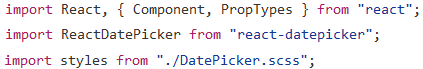
\includegraphics[scale=0.9]{figure/imports.png}
    \caption{The needed importations for the DatePicker UI component.}
    \label{fig:imports}
\end{figure}

This last imported file contains the local CSS styles for the date picker, that will not be used anywhere else in the application. Local classes are applied to the component by using \{styles.className\}, where \textit{className} refers to the name of the wanted class. Such CSS modules group all the styles per component, and make sure that changes made in the CSS for one UI component will not affect the other ones~\cite{localCSS}.

However, Konnektid also uses global CSS variables (for fonts, colors, and so on) that are defined in .scss files at the root of the ui folder. They are default values meant to be reused in every component, inside the local classes, to make the website more harmonious. With them I could customize react-datepicker, and the final result is presented on {\sc figure}~\ref{fig:datePicker}. It now features the Konnektid default font, and some recurrent colors of the application (specific green and purple).

\begin{figure}[H]
    \centering
    
\includegraphics[scale=0.6]{figure/datePicker.png}
    \caption{The final DatePicker presentational component.}
    \label{fig:datePicker}
\end{figure}

This assignment was an efficient way to learn JavaScript and some good ReactJS practices. Moreover, it was a great introduction to the ReactJS community and all the support that it brings, especially with the numerous free plugins that are shared.

It is important here to note that the pages that already existed on the website do not use this new library of UI components. Instead of rebuilding them all, which would have been terribly time-consuming, we were able to keep them in separate folders: \textit{public} for public pages such as the homepage, \textit{app} for private pages~\footnote{Pages accessible only when the user is logged in.} such as the activity feed. They are now referred to as \guillemotleft{} old \guillemotright{} pages whereas the most recent pages, built with the UI library, are called \guillemotleft{} new \guillemotright{}.

\subsection{Implementation of new pages}
\label{ssec:new_pages}

It has been explained in {\sc subsection}~\ref{ssec:concept} that Konnektid's main goal for the year is to test and validate their business model, which relies on
professional teachers. This requires the implementation of several new pages and functionalities, and lots have been built during the internship. Among them, one will be described here: the course page.

It refers to the page used by teachers to create, edit and publish a course. It had to be built from scratch, for both desktop and mobile, based on designs
made by Konnektid's former designer. It is now released and used by professional teachers, and a desktop example is visible in {\sc attachment}~\ref{sec:courseDesktop}.

The page features two main elements:

\textbf{The top section} which contains the main information about the course (picture, title, price\ldots) and the teacher (avatar, name\ldots).
The teacher name is a direct link to his or her profile. This section also provides a button \guillemotleft{} Enroll now \guillemotright{} for the students to book the course.

\textbf{The bottom section} which is divided in two parts. The right part takes most space on the page and gives an in-depth description of the course
(methodology, requirements\ldots). The left part, thinner, shows practical information about the course (format, length\ldots) and another \guillemotleft{} Enroll now \guillemotright{} button with a reminder of the price. Below this are the sharing functionalities: Facebook, Twitter,
email, and WhatsApp on mobile.

The initial step in the implementation was to create the corresponding route, to indicate that \url{https://www.konnektid.com/course/:id} (where \textit{id} is the course identifier) leads to the \guillemotleft{} Course \guillemotright{} route handler. It is a JavaScript file rendering the Course component inside of the website layout. Later on, when the UI is finished and the logic is added using Redux, the route handler renders the Course container instead of the component.

To build the Course component, the first challenge was to decide how to divide it in sub-components, each of them implemented in their own folder with local CSS styles as explained in {\sc subsection}~\ref{ssec:ui_components}. For instance, the biggest bottom part shown on {\sc figure}~\ref{fig:courseDescription} is a component called \guillemotleft{} CourseDescriptionCard \guillemotright{}.

\begin{figure}[H]
    \centering
    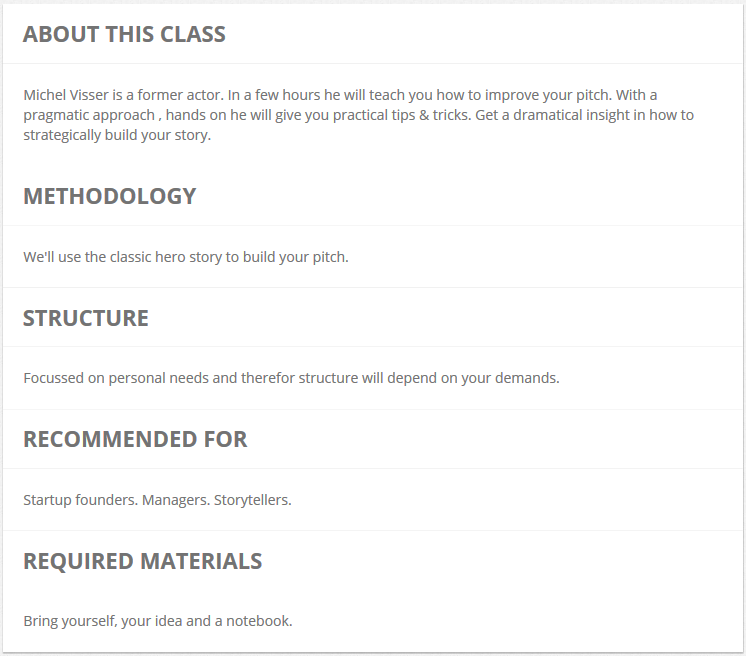
\includegraphics[scale=0.6]{figure/courseDescription.png}
    \caption{An example of course description, in the bottom part of the course page.}
    \label{fig:courseDescription}
\end{figure} 

We can see that it contains several sections, that are similar in presentation and only differ by their title and content. So
it made sense to create a reusable \guillemotleft{} CourseDescriptionItem \guillemotright{} sub-component, to render each of them with title and content passed down as properties. This reasoning respects the single responsibility principle previously mentioned in {\sc subsection}~\ref{ssec:frameworks} and avoids duplicated code.
These are two of the many good practices for writing maintainable code~\cite{maintainable}, i.e. code that is easy to read, to modify and to extend.

After finishing the interface of the page, I was asked to add inline editing features to it. This means that elements can be edited in-place, in the context where they will be published. I used an editor framework for ReactJS called \textit{DraftJS}, which enables the creation of rich content such as bold/italic text or lists of items~\cite{draftJS}. An example of editable CourseDescriptionItem component is displayed on {\sc figure}~\ref{fig:courseEdit}. When mousing over the content, a gray frame appears around it to draw attention, and the teacher can just click on it to start writing as explained by the green tip on top. For now it is empty, so the placeholder \guillemotleft{} If you leave this empty... \guillemotright{} is displayed.

\begin{figure}[H]
    \centering
    
\includegraphics[scale=0.4]{figure/courseEdit.png}
    \caption{One of the course description items in edition mode.}
    \label{fig:courseEdit}
\end{figure}

DraftJS is based on an \guillemotleft{} Editor \guillemotright{} component, whose state is stored in an \guillemotleft{} EditorState \guillemotright{} object holding all the information about the content: the text and its decoration (bold, italic\ldots), the selection\ldots A method \textit{onChange}, passed down as property, is called to update the state every time the user changes the content of the editor. Moreover, it is possible to define customized key bindings, by using the \textit{keyBindingFn} and \textit{handleKeyCommand} properties. The first function returns a command string depending on the pressed key, then the second one takes that string as input and outputs the corresponding changes on the editor content.

This page was the first static page I fully created, and it made me realize how useful the components library mentioned in {\sc subsection}~\ref{ssec:ui_components} is. I had a lot of similar requirements during the traineeship, so at the end I was able to quickly deliver well-structured frontend pages, and even UI for entire flows such as booking a course with online payment.

\subsection{Refactoring of existing pages}
\label{ssec:refactor}

Adding funtionalities to the website sometimes involve updating old pages, usually with small changes: for example, I actualized the professional teachers presented on the homepage, in the \guillemotleft{} Book a professional teacher \guillemotright{} section, to highlight the newly released teacher profiles and course pages. In this case, revising the former code was enough. But sometimes, a whole refactoring is needed, and then the best option is to entirely rebuild the page using the UI library. 

This is what happened for the teachers landing page, which describes Konnektid's offer for professional teachers in order to convince people to become one. It has been decided to improve it, because the conversion rate (i.e. the number of users signing up as teachers compared to the number of visitors of the page, obtained via the analytics) was not satisfying. 

To get started, we had a brainstorm session to determine what contents were needed, and how they should be structured. We came up with a wireframe\footnote{Basic skeleton of the page, representing the main UI elements and how they work together.}, and since there was no designer back then, this was the only support I had for development. So I quickly built and presented a first draft, to make sure I was heading in the right direction and to get a first round of feedback.

Based on this, I could iterate the process and gradually improve the interface until it was validated, for both desktop and phone. Then, to verify that we were sending the right message, the copywriting was reviewed together with the community manager. She also helped me out by collecting quotes from current professional teachers, who were then integrated in the page as social proof of the concept. This first version was released in \textit{alpha}. A while later, a designer joined the team and suggested a few modifications concerning the User Experience (UX) and the UI of the page, so we worked together on improving it. 

In the meantime, the registration process for professional teachers was also being refactored, but it was not yet ready. So I had to implement a temporary sign-up flow, based on the former one visible on {\sc figure}~\ref{fig:signUpFlow}.

 \begin{figure}[H]
    \centering
    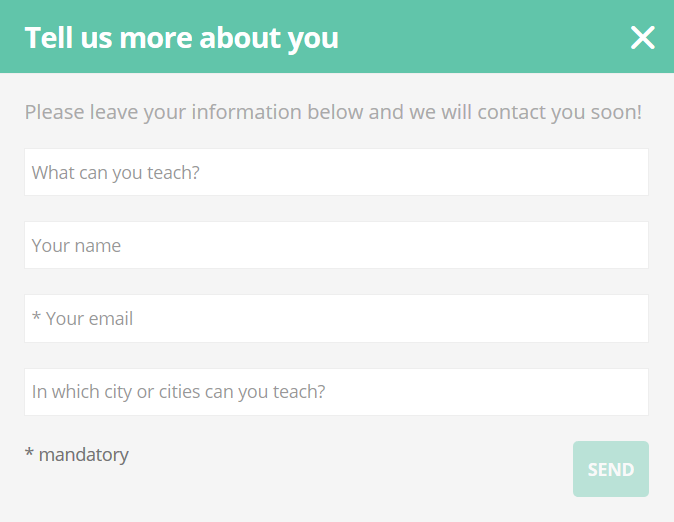
\includegraphics[scale=0.6]{figure/signUpFlow.png}
    \caption{The registration form for professional teachers.}
    \label{fig:signUpFlow}
\end{figure}

It is a modal with four fields to fill in: the name and email of the applicant, the skill(s) to teach, and the city or cities where he/she could teach. When clicking on \guillemotleft{} Send \guillemotright{}, an email is sent to the Konnektid team with all the provided information. If everything goes well, a new screen appears to indicate the success, and the request can be treated by Konnektid (i.e. get in touch with the person, verify the certifications\ldots). If there is a problem (for instance while sending the email), an error screen appears to inform the applicant that the request could not be sent.

I had to re-create this modal with the UI components of the new library, as a component called \guillemotleft{} BecomeTeacherModal \guillemotright{}. It contains a form (\guillemotleft{} BecomeTeacherForm \guillemotright{}) receiving the screen as property, which can have three values: \guillemotleft{} form \guillemotright{}, \guillemotleft{} success \guillemotright{} or \guillemotleft{} error \guillemotright{}. It also has a container to manage the state of the modal (i.e. when to show it or not) and of the form (i.e. which screen to display) thanks to a Redux reducer that I implemented along with its tests. The form itself was built with \textit{redux-form}, a plugin specially designed for managing form state in React using Redux.

I used redux-form in the container on top of the BecomeTeacherForm component, to perform all the necessary verifications needed to validate the form. For example, the email address is mandatory, and also needs to respect a certain format (e.g. test@test.com). The code of the BecomeTeacherForm container, testing the email value, can be seen on {\sc figure}~\ref{fig:reduxForm} where \textit{isEmail} is a utility checking the email format.

 \begin{figure}[H]
    \centering
    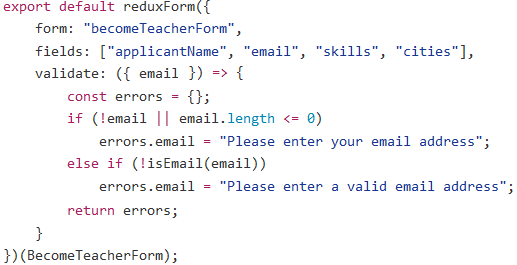
\includegraphics[scale=0.8]{figure/reduxForm.png}
    \caption{The BecomeTeacherForm container, using redux-form.}
    \label{fig:reduxForm}
\end{figure}

Then, the error to display (if any) and the validation of the email can be used in the component, respectively via \textit{email.error} and \textit{email.valid}. The error will appear in red under the corresponding input, to inform the user that something is wrong and give improvement indications. The validation is used to able or not the \guillemotleft{} Send \guillemotright{} action, as on {\sc figure}~\ref{fig:signUpFlow} where the button is disabled because the email field is empty.

The remaining task for this project was to create a GraphQL mutation to notify Konnektid of the registration request. To do so, I started by creating \guillemotleft{} notifyRegisteredTeacherMutation.js \guillemotright{}, which takes as input a \guillemotleft{} TeacherRegistration \guillemotright{} object containing all the fields of the form and their values. When \guillemotleft{} Send \guillemotright{} is clicked, the mutation is called in the \guillemotleft{} becomeTeacherModal \guillemotright{} reducer, via the \textit{completeRegistrationProcess} method visible on {\sc figure}~\ref{fig:completeRegistration}.

 \begin{figure}[H]
    \centering
    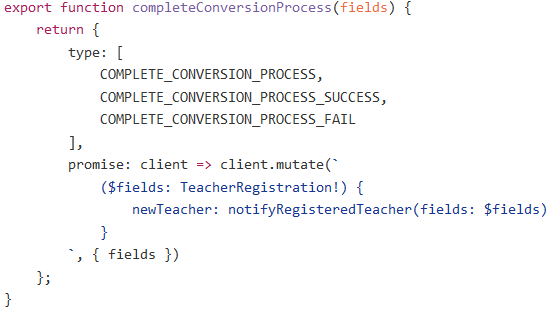
\includegraphics[scale=0.8]{figure/completeRegistration.png}
    \caption{The function handling the registration request.}
    \label{fig:completeRegistration}
\end{figure}

This asynchronous function fires the \textit{COMPLETE\_REGISTRATION\_PROCESS} action, and if the mutation is successful sends \textit{COMPLETE\_REGISTRATION\_PROCESS\_SUCCESS}, updating the screen to \guillemotleft{} success \guillemotright{}. Otherwise, \textit{COMPLETE\_REGISTRATION\_PROCESS\_FAIL} is returned and the screen becomes \guillemotleft{} error \guillemotright{}.

Then, in \guillemotleft{} notifyRegisteredTeacherMutation.js \guillemotright{}, I had to handle three things: 
\begin{itemize}[noitemsep]
    \item Internally send an email to the Konnektid team, to inform them of the registration request;
    \item Create a task in Asana with the applicant's data, in a dedicated project;
    \item Send an email to the teacher-to-be, as a confirmation that the request has been sent.
\end{itemize}

The final desktop version of the new teachers landing page is available in {\sc attachment}~\ref{sec:teachersPage}. It was great to follow the creation process from A to Z, and to be fully responsible for it, even if it was challenging to build everything from scratch with technologies I had never used before.

\subsection{New navigation}
\label{ssec:new_nav}

After discussions with the designer, it appeared that the navigation in the private pages of the application was unclear and too complicated. So, it has been decided to refactor it, and I took care of the implementation (both in mobile and desktop) based on design mockups. I will only describe the process for the old pages, as the one for new pages is basically the creation of UI components, and it is already detailed in {\sc subsection}~\ref{ssec:ui_components}.

First, since this is a consequent change, I created a feature flag (trick described in {\sc subsection}~\ref{ssec:env}) named \guillemotleft{} new\_navigation\_enabled \guillemotright{}. I set it to true in the \textit{development} and \textit{alpha} configuration files, but to false in \textit{production}. This means that no matter what happens, the changes will only appear in \textit{alpha} and will not affect \textit{production} (the actual website). I also added it to \guillemotleft{} legacyConfig.js \guillemotright{}, visible on {\sc figure}~\ref{fig:legacyConfig}, which takes the configuration for new pages and converts it into configuration for old pages.

\begin{figure}[H]
    \centering
    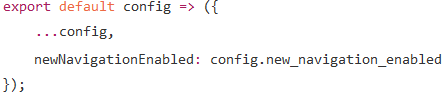
\includegraphics[scale=0.8]{figure/legacyConfig.png}
    \caption{The content of \textit{legacyConfig.js}.}
    \label{fig:legacyConfig}
\end{figure}

This configuration can then be passed down to components as \guillemotleft{} config \guillemotright{} property, thanks to a helper called \textit{connectLegacyConfig}. The feature flag is then accessed via \textit{this.props.config.newNavigationEnabled} and needs to be checked at every code modification, to be certain that changes will be applied only if this flag is set to true.

Since it is usually difficult to dive into existing code and modify it, especially if somebody else wrote it, I started by updating the old pages. This code is not as structured as the one for new pages, because it does not use presentational components nor local CSS styles. Instead, it features a lot of stateful components, and global CSS files stored in a separate \guillemotleft{} styles \guillemotright{} folder. These files contain lots of classes, most of them being used in several components, and this really makes CSS styles harder to find and to understand. 

In desktop, I thought that the changes would be quite fast to make as the former header ({\sc figure}~\ref{fig:oldNavDesktop}) was relatively similar to the new one ({\sc figure}~\ref{fig:newNavDesktop}). But it turned out to be more complex than expected.

\begin{figure}[H]
    \centering
    
\includegraphics[scale=0.3]{figure/oldNavDesktop.png}
    \caption{The former private header for desktop.}
    \label{fig:oldNavDesktop}
\end{figure}

\begin{figure}[H]
    \centering
    
\includegraphics[scale=0.47]{figure/newNavDesktop.png}
    \caption{The refactored private header for desktop.}
    \label{fig:newNavDesktop}
\end{figure}

The old header was generated based on \guillemotleft{} private-menu.js \guillemotright{}, a file containing all its elements shaped as objects with two fields: the label to display (e.g. \guillemotleft{} My requests \guillemotright{}) and the associated URL (e.g. \guillemotleft{} /requests \guillemotright{}). I had to rebuild this file, as \guillemotleft{} new-private-menu.js \guillemotright{}, to remove unused sections and to include the icons, found in the Font Awesome library~\footnote{http://fontawesome.io/icons/}. For this, I added to each object a field called \guillemotleft{} icon \guillemotright{}, as seen on {\sc figure}~\ref{fig:icon}. 

\begin{figure}[H]
    \centering
    
\includegraphics[scale=0.9]{figure/icon.png}
    \caption{An object of \textit{new-private-menu.js}.}
    \label{fig:icon}
\end{figure}

The icon itself is then defined for each menu item in a span HTML tag, by setting its className property (i.e. its CSS styles) as pictured on {\sc figure}~\ref{fig:classnames}, using a utility called \textit{classnames}~\footnote{https://github.com/JedWatson/classnames} (referred to as \guillemotleft{} cn \guillemotright{} on the figure). This method takes several CSS classes, and blends them into one, sometimes under certain conditions. Here for instance, it combines \guillemotleft{} fa \guillemotright{} which points out to the Font Awesome library, \guillemotleft{} fa-lg \guillemotright{} which defines the size of the icon, and \guillemotleft{} fa-\$\{item.icon\} \guillemotright{} which indicates the icon to display (it would be \guillemotleft{} fa-graduation-cap \guillemotright{} for the object on {\sc figure}~\ref{fig:icon}). 

\begin{figure}[H]
    \centering
    
\includegraphics[scale=0.9]{figure/classnames.png}
    \caption{The definition of the menu icons.}
    \label{fig:classnames}
\end{figure}

Once this was done, I had to implement the \guillemotleft{} My activities \guillemotright{} header section, and its dropdown visible on {\sc figure}~\ref{fig:newNavDesktop}. I created a new component for it (\guillemotleft{} KndActivitiesMenu \guillemotright{}) and a CSS class (\textit{activities-menu}) to place it relatively to the last header section. This also involved a few changes in the last section's CSS class (\textit{navatar-menu}). The activities menu was then included inside the \guillemotleft{} KndPrivateHeader \guillemotright{} component, as seen on {\sc figure}~\ref{fig:activitiesImpl}, where \textit{renderActivitiesMenu()} renders the KndActivitiesMenu component.

\begin{figure}[H]
    \centering
    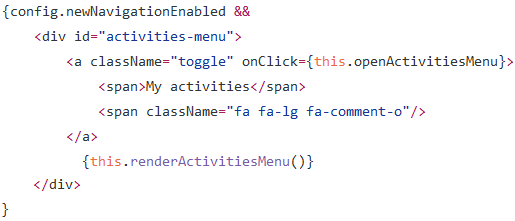
\includegraphics[scale=0.9]{figure/activitiesImpl.png}
    \caption{The implementation of the activities menu.}
    \label{fig:activitiesImpl}
\end{figure}

Finally, KndPrivateHeader is stateful, and handles by itself the logic of showing (or not) the dropdowns it contains. It already had in its state a variable named \guillemotleft{} showProfileMenu \guillemotright{}, used to handle the profile dropdown. This variable is updated by calling either \textit{closeProfileMenu()} or \textit{openProfileMenu()}, fired when clicking on the user's name. To be able to toggle the new activities menu, I extended the state with \guillemotleft{} showActivitiesMenu \guillemotright{}, and implemented the related methods \textit{closeActivitiesMenu()} and \textit{openActivitiesMenu()}.

After updating the desktop navigation, I worked on the mobile one (still in old pages). This time, it was completely different from the old version: it used to be a burger button on the top left, toggling an offcanvas menu with all the possible sections. Now it is a header with full-width dropdowns, as shown on {\sc figure}~\ref{fig:newNavPhone}. I thought this would be harder to implement than the desktop version, but in the end it was actually faster because it did not involve a lot of modification in the code, but mainly addition.

\begin{figure}[H]
    \centering
    
\includegraphics{figure/newNavPhone.png}
    \caption{The new private navigation for phone.}
    \label{fig:newNavPhone}
\end{figure}

First, I created a static version (\guillemotleft{} KndPrivateMobileMenu \guillemotright{}), without the dropdowns, and its corresponding CSS class (\textit{mobile-main-menu}). It was then integrated to KndPrivateHeader via \textit{renderMobileHeader()}, with a previous check of the flag, similarly to the desktop activities menu previously described.

Then, I built the dropdowns, respectively added to KndPrivateHeader via \textit{renderMobileActivitiesMenu()} and \textit{renderMobileProfileMenu()}. Since they both show up full-width under the header, I created a wrapper CSS class for them (\textit{mobile-menu-wrapper}) to define this behavior. Finally, I had to expand the state again, by adding the \guillemotleft{} showMobileProfileMenu \guillemotright{} and \guillemotleft{} showMobileActivitiesMenu \guillemotright{} variables, along with their corresponding opening and closing functions. 

I was responsible for this new navigation project, which means that I had to keep the other developers informed of the progress by regular status updates. Once it was finished, I organized a demonstration for it, so that the whole team could see it and give feedback. Unfortunately, the comments were not all positive, and some of the changes had to be reversed. For the developers team, it was a reminder to always validate the design mockups with the rest of the team before implementing them. Personnally, this experience taught me to take responsability for the code I produce, and to accept critics on it despite the time spent to write it.

\subsection{Web analytics}
\label{ssec:analytics}

Web analytics consist in collecting all the details about a website's usage (e.g. which buttons are most clicked) and traffic (e.g. how many page views per day). Konnektid mainly uses them as a market research tool, to gather information about the users and their experience with the web application. Almost all possible interactions on the platform are tracked: this data is then analyzed, to determine where improvements are needed but also to provide statistics as proof of the business model. 

If it is decided to refactor an existing feature, analytics help to test whether the changes actually had an impact, and if it is a positive one. This process can be iterated until satisfying results are obtained. Also, after the addition of a new functionality, analytics provide valuable insights on how often it is used, how well it achieves its goals, and how it should be enhanced.

During my internship, I had to implement the analytics in the new pages, from a list of all the related events that needed to be tracked. I will here describe the building process for only one of them: make a booking from a course page. 

Analytics in new pages are closely related to the Redux actions introduced in {\sc subsection}~\ref{ssec:tools}. Indeed, when a user interacts with the website, a corresponding Redux action is created and along with it an analytics event is fired. For example, if a member decides to book a course with a professional teacher, he confirms it by clicking an \guillemotleft{} Enroll \guillemotright{} button. As soon as this is done, the function \textit{completeEnrollProcess} from {\sc figure}~\ref{fig:enroll} is called.

\begin{figure}[H]
    \centering
    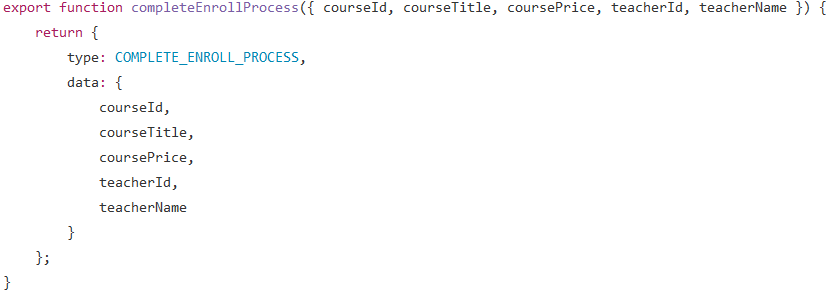
\includegraphics[scale=0.9]{figure/enroll.png}
    \caption{The action creator called when a user books a course.}
    \label{fig:enroll}
\end{figure}

This function is a Redux action creator: it returns a Redux action, containing a type (\guillemotleft{} COMPLETE\_ENROLL\_PROCESS \guillemotright{}) and some data (course id, teacher id\ldots). The action is then mapped to the analytics by the \textit{mapActionsToAnalytics} function, visible on {\sc figure}~\ref{fig:mapActions}.

\begin{figure}[H]
    \centering
    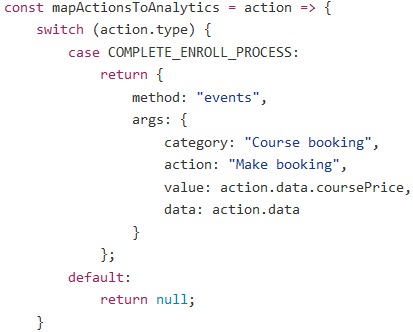
\includegraphics[scale=0.9]{figure/mapActions.png}
    \caption{The function mapping Redux actions to analytics.}
    \label{fig:mapActions}
\end{figure}

The returned object contains two fields, the method (always \guillemotleft{} events \guillemotright{} no matter the action) and the args. The args represent the data needed for the analytics, that will be displayed and analyzed by two tools: 

\textbf{Google Analytics} offering numerous services: calculation of conversion rates, estimation of sales, information on used devices\ldots Plus, it provides help for marketing and advertising~\cite{googleAnalytics}. 

\textbf{Mixpanel} focusing on funnels, i.e. visual representations of how users move through a series of events. This aims at finding out where users abandon and why~\cite{mixpanel}.

In old pages, analytics sometimes need to be improved, either when an extra information requires measurement or when an existing functionality has been modified. This was the case when I added an \guillemotleft{} Invite friends \guillemotright{} call-to-action (\guillemotleft{} CTA \guillemotright{}) after a member offered to teach somebody (screen on {\sc figure}~\ref{fig:afterOffer}).

\begin{figure}[H]
    \centering
    
\includegraphics[scale=0.8]{figure/afterOffer.png}
    \caption{The screen appearing after making an offer, now with an Invite friends button.}
    \label{fig:afterOffer}
\end{figure}

Konnektid wanted to track the clicks on this new CTA, to compare its performance to the other Invite friends buttons dispatched on the website. So, I had to figure out how the analytics are fired in the old pages, that do not use Redux.

Instead, a helper called \textit{connectAnalytics} passes down the \textit{analytics} property to the component, that is then accessed via \textit{getAnalytics()}. It contains a certain number of methods, each one corresponding to a possible event. In this case I used an existing one, \textit{inviteFriendsClicked}. It takes as parameter a constant representing the source of the event, i.e. from where in the application it has been fired. The possible values for this constant are defined inside the \guillemotleft{} constants \guillemotright{} folder, in \guillemotleft{} InviteFriendsConstants.js \guillemotright{}. This file contains all possible sources for the Invite friends event, so I added \guillemotleft{} AFTER\_OFFER \guillemotright{} to it, as visible on {\sc figure}~\ref{fig:inviteFriendsConstants}.

\begin{figure}[H]
    \centering
    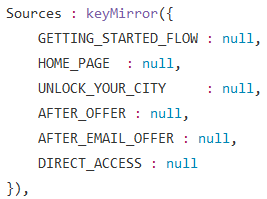
\includegraphics[scale=0.9]{figure/inviteFriendsConstants.png}
    \caption{All the possible sources for the \guillemotleft{} Invite friends \guillemotright{} event.}
    \label{fig:inviteFriendsConstants}
\end{figure}

I could then define \textit{inviteClicked()} ({\sc figure}~\ref{fig:inviteClicked}), which is fired every time a user clicks on Invite friends after making an offer. It sends the event to the analytics. 

\begin{figure}[H]
    \centering
    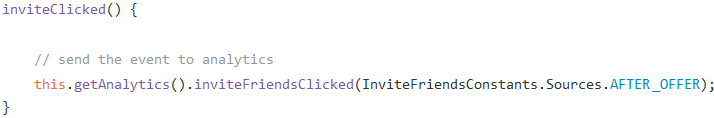
\includegraphics[scale=0.9]{figure/inviteClicked.png}
    \caption{The \textit{inviteClicked()} method, used to send analytics.}
    \label{fig:inviteClicked}
\end{figure}

Analytics are very important for Konnektid, and for web applications in general, so it was great to be able to manipulate them and understand how they work. It was a whole new concept to me, and I was impressed to see how they are used, not only to enhance the website's UX/UI but also to prove the business model. Implementation-wise, it was especially interesting in the new pages, because using Redux for analytics is a rather modern technique.

\subsection{New application}
\label{ssec:newApp}

At the beginning of August, it has been decided to split the Konnektid application into two websites: one focused on free use and community building, and the other containing the market place (i.e. professional teachers and course offering) for members willing to pay for learning. 

A whole new Git repository has been created, with all the required infrastructure, including the UI components library. Some of my last achievements as a trainee were frontend pages for the new website, such as the homepage ({\sc attachment}~\ref{sec:newHome}). I also implemented user interfaces for entire flows, like \guillemotleft{} Find a teacher \guillemotright{}: it is a new functionality, proper to the market place, which allows members to specify what they want to learn and how (for instance, private or group classes) so that Konnektid can find a suitable teacher for them.

Technically speaking, these tasks were not particularly challenging as they were similar to the ones described in {\sc subsections}~\ref{ssec:ui_components} and ~\ref{ssec:new_pages}. But the creation of this second website made me realize how fast startups evolve, and how decisive choices must sometimes be made when building a company. It is important to be adaptable, creative, and not afraid to try out lots of solutions before succeeding, when working in such a changing environment.

    \newpage
    \section{General conclusion}
\label{sec:conclusion}

This traineeship has been a very rich experience, for many reasons that have been detailed in the previous sections and that are summarized here in the general conclusion.

Technically, it brought me a lot of knowledge in a discipline that I had not experienced before: web development, and more specifically single-page applications. I have improved my skills in languages such as JavaScript, HTML and SCSS, and understood the concepts of frontend and backend development. I learned the main good practices and principles for writing clean, understandable, maintainable code, and got to use some modern frameworks and libraries (ReactJS, Redux, GraphQL and more). This increased my curiosity about new technologies, and I got the chance to attend some very interesting conferences about them. 

Moreover, I now know better how to use Github as a communication tool for technical issues, and how to deal with local branches, pull requests and multi-environmental development. Plus, I discovered the concept of feature flag, an insurance that critical changes will not affect other branches.

Being part of a small team made me realize the importance of communication and collaboration in project management. I especially often worked with the designer and the community manager, which was also the occasion to learn more about their job and skillset. And since Konnektid is currently trying to prove their business model as a market place, I discovered the techniques that you can use to do so: web analytics, marketing tools, etc.

From the company point of view, I believe that I produced a lot of value in terms of new features built and improvements. I was quickly able to deliver new frontend pages and components with good quality code and intelligent structure. I learned how to be independant and was able to decide by myself which task to start next, depending on the month's objectives for Konnektid. I was also involved in brainstorming sessions and meetings where my opinion and ideas were truly appreciated.

As a conclusion, the most valuable asset for me was to get assigned to many different tasks, from building interfaces to implementing analytics or creating wireframes. It really made me think about what I like, and what I want to do after the internship.

    \newpage
    \section{Attachments}
\label{sec:attach}

\subsection{Global planning}
\label{ssec:planning}

{\sc table}~\ref{table:planning} presents an overview of the main development achievements of the internship, per month. Many smaller tasks have been omitted, as well as the meetings, demonstrations and brainstorming sessions that were also an important part of the planning.

\bgroup
	\def\arraystretch{1.5}
		\begin{table}[H]
		\centering
			\begin{tabular}{|l|l|}
			\hline
			\textbf{March} & \begin{tabular}[c]{@{}l@{}}Setup and tool discovery\\ Lots of small tasks (copywriting, debugging, emails improvement...)\\ Addition of scrolling button in activity feed \\ Privacy statement update\\ Creation of User terms page\end{tabular} \\ \hline
			\textbf{April} & \begin{tabular}[c]{@{}l@{}}Creation of Unlock your city email\\ Account deletion modal improvement\\ UI components building (Label, Alert...)\\ Course page UI implementation, with inline editing\end{tabular} \\ \hline
			\textbf{May} & \begin{tabular}[c]{@{}l@{}}Implementation of reviewing process for teachers\\ Handling non-existing pages and URLs\\ Global public/private layout refactoring\\ Mobile menu fixing (close on outside click)\end{tabular} \\ \hline
			\textbf{June} & \begin{tabular}[c]{@{}l@{}}Wireframing for matchmaking flow\\ UI components building (date and time pickers)\\ Overall navigation refactoring\\ Analytics addition to new pages\end{tabular} \\ \hline
			\textbf{July} & \begin{tabular}[c]{@{}l@{}}New teachers landing page creation\\ SEO improvement for /courses page\\ Booking flow with payment UI building\end{tabular} \\ \hline
			\textbf{August} & \begin{tabular}[c]{@{}l@{}}Administrator UI implementation\\ Temporary sign-up flow addition to new teachers page\\ Modal UI component refactoring\\ Find teacher flow UI building\end{tabular} \\ \hline
			\end{tabular}
		\label{table:planning}
		\end{table}
\egroup

\newpage

\subsection{A course published on Konnektid's website (desktop version)}
\label{ssec:courseDesktop}

\begin{figure}[H]
    \centering
    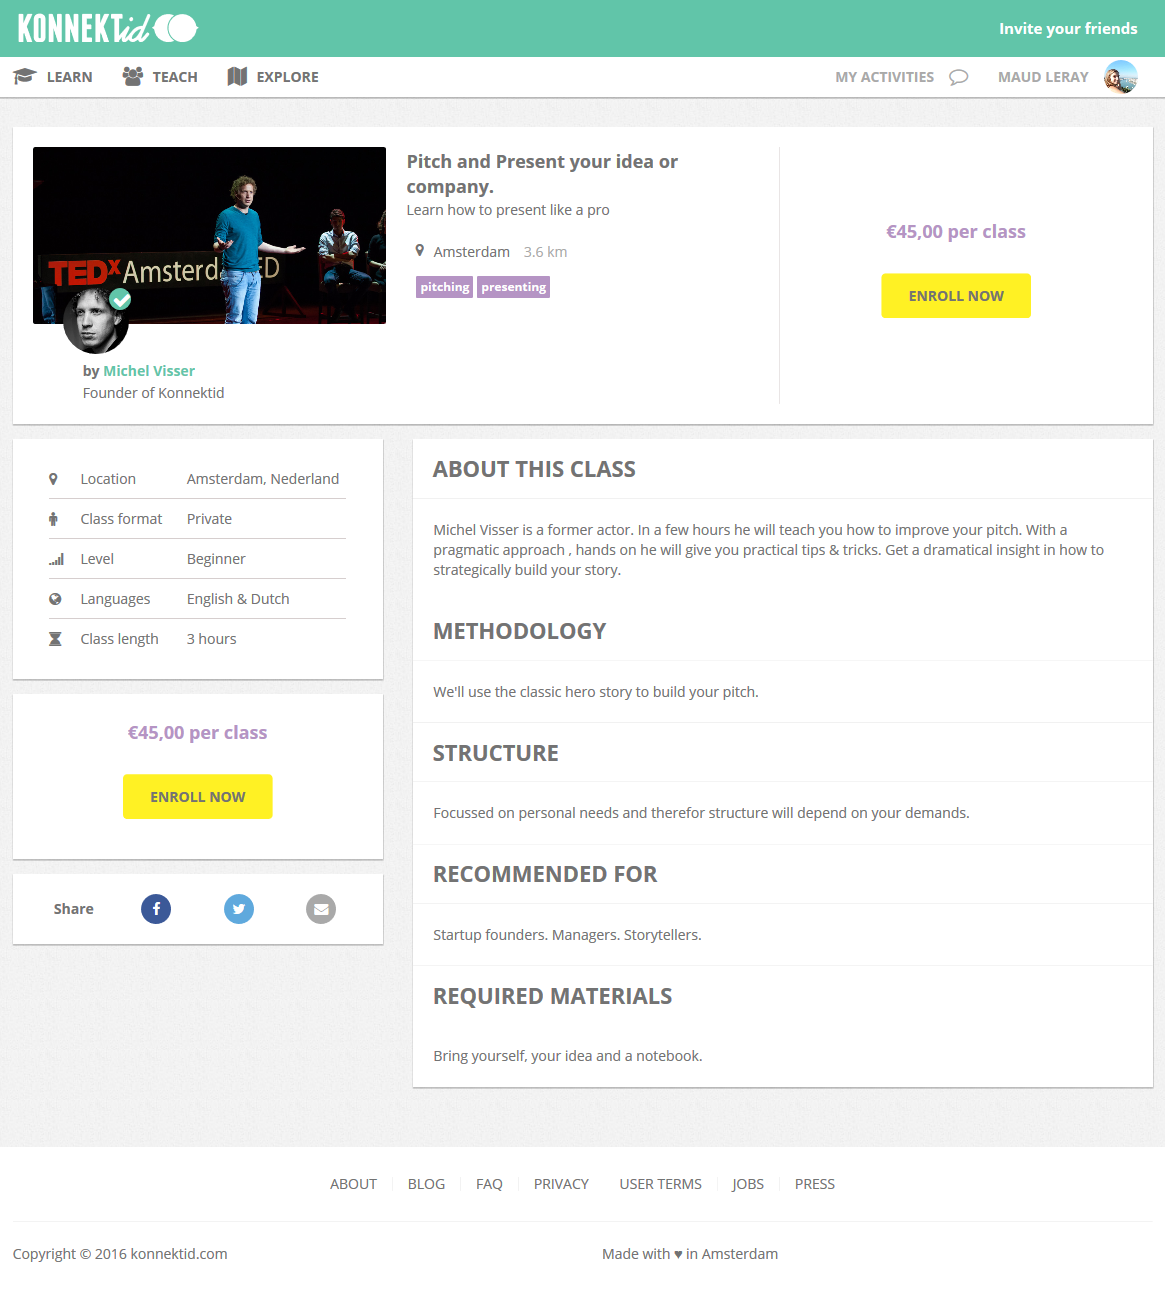
\includegraphics[scale=0.6]{figure/coursePage.png}
\end{figure}

\newpage

\subsection{The refactored teachers landing page (desktop version)}
\label{ssec:teachersPage}

\begin{figure}[H]
    \centering
    
\includegraphics[scale=0.1]{figure/teachersPage.png}
\end{figure}

\newpage

\subsection{The homepage for the new market place (desktop version)}
\label{ssec:newHome}

\begin{figure}[H]
    \centering
    \includegraphics[scale=0.1]{figure/newHome.png}
\end{figure}


    \emptypage
    \newpage
    \bibliographystyle{plain}
    \newpage
    \bibliography{input/biblio}

    \emptypage
    \ifthenelse{\isodd{\thepage}}
    {\emptypage}
    {}
    
\includepdf[page=2]{figure/cover.pdf}
\end{document}
